\documentclass[conference,letterpaper,final]{IEEEtran}
% Add the compsoc option for Computer Society conferences.
%
% If IEEEtran.cls has not been installed into the LaTeX system files,
% manually specify the path to it like:
% \documentclass[conference]{../sty/IEEEtran}
\special{papersize=8.5in,11in}






% *** CITATION PACKAGES ***
%
\usepackage{cite}




% *** GRAPHICS RELATED PACKAGES ***
%
\ifCLASSINFOpdf
  % \usepackage[pdftex]{graphicx}
  % declare the path(s) where your graphic files are
  % \graphicspath{{../pdf/}{../jpeg/}}
  % and their extensions so you won't have to specify these with
  % every instance of \includegraphics
  % \DeclareGraphicsExtensions{.pdf,.jpeg,.png}
\else
  % or other class option (dvipsone, dvipdf, if not using dvips). graphicx
  % will default to the driver specified in the system graphics.cfg if no
  % driver is specified.
   \usepackage[dvips]{graphicx}
  % declare the path(s) where your graphic files are
  % \graphicspath{{../eps/}}
  % and their extensions so you won't have to specify these with
  % every instance of \includegraphics
  % \DeclareGraphicsExtensions{.eps}
\fi




% *** MATH PACKAGES ***
%
\usepackage[cmex10]{amsmath}



% *** SPECIALIZED LIST PACKAGES ***



% *** ALIGNMENT PACKAGES ***
%
%\usepackage{array}
% Frank Mittelbach's and David Carlisle's array.sty patches and improves
% the standard LaTeX2e array and tabular environments to provide better
% appearance and additional user controls. As the default LaTeX2e table
% generation code is lacking to the point of almost being broken with
% respect to the quality of the end results, all users are strongly
% advised to use an enhanced (at the very least that provided by array.sty)
% set of table tools. array.sty is already installed on most systems. The
% latest version and documentation can be obtained at:
% http://www.ctan.org/tex-archive/macros/latex/required/tools/


%\usepackage{mdwmath}
%\usepackage{mdwtab}
% Also highly recommended is Mark Wooding's extremely powerful MDW tools,
% especially mdwmath.sty and mdwtab.sty which are used to format equations
% and tables, respectively. The MDWtools set is already installed on most
% LaTeX systems. The lastest version and documentation is available at:
% http://www.ctan.org/tex-archive/macros/latex/contrib/mdwtools/



% *** SUBFIGURE PACKAGES ***
%\usepackage[tight,footnotesize]{subfigure}
% subfigure.sty was written by Steven Douglas Cochran. This package makes it
% easy to put subfigures in your figures. e.g., "Figure 1a and 1b". For IEEE
% work, it is a good idea to load it with the tight package option to reduce
% the amount of white space around the subfigures. subfigure.sty is already
% installed on most LaTeX systems. The latest version and documentation can
% be obtained at:
% http://www.ctan.org/tex-archive/obsolete/macros/latex/contrib/subfigure/
% subfigure.sty has been superceeded by subfig.sty.



%\usepackage[caption=false]{caption}
%\usepackage[font=footnotesize]{subfig}
% subfig.sty, also written by Steven Douglas Cochran, is the modern
% replacement for subfigure.sty. However, subfig.sty requires and
% automatically loads Axel Sommerfeldt's caption.sty which will override
% IEEEtran.cls handling of captions and this will result in nonIEEE style
% figure/table captions. To prevent this problem, be sure and preload
% caption.sty with its "caption=false" package option. This is will preserve
% IEEEtran.cls handing of captions. Version 1.3 (2005/06/28) and later 
% (recommended due to many improvements over 1.2) of subfig.sty supports
% the caption=false option directly:
%\usepackage[caption=false,font=footnotesize]{subfig}
%
% The latest version and documentation can be obtained at:
% http://www.ctan.org/tex-archive/macros/latex/contrib/subfig/
% The latest version and documentation of caption.sty can be obtained at:
% http://www.ctan.org/tex-archive/macros/latex/contrib/caption/




% *** FLOAT PACKAGES ***
%
\usepackage{fixltx2e}
\usepackage[hmargin=1in,vmargin=1in]{geometry}
%\usepackage{fullpage}
% fixltx2e, the successor to the earlier fix2col.sty, was written by
% Frank Mittelbach and David Carlisle. This package corrects a few problems
% in the LaTeX2e kernel, the most notable of which is that in current
% LaTeX2e releases, the ordering of single and double column floats is not
% guaranteed to be preserved. Thus, an unpatched LaTeX2e can allow a
% single column figure to be placed prior to an earlier double column
% figure. The latest version and documentation can be found at:
% http://www.ctan.org/tex-archive/macros/latex/base/



%\usepackage{stfloats}
% stfloats.sty was written by Sigitas Tolusis. This package gives LaTeX2e
% the ability to do double column floats at the bottom of the page as well
% as the top. (e.g., "\begin{figure*}[!b]" is not normally possible in
% LaTeX2e). It also provides a command:
%\fnbelowfloat
% to enable the placement of footnotes below bottom floats (the standard
% LaTeX2e kernel puts them above bottom floats). This is an invasive package
% which rewrites many portions of the LaTeX2e float routines. It may not work
% with other packages that modify the LaTeX2e float routines. The latest
% version and documentation can be obtained at:
% http://www.ctan.org/tex-archive/macros/latex/contrib/sttools/
% Documentation is contained in the stfloats.sty comments as well as in the
% presfull.pdf file. Do not use the stfloats baselinefloat ability as IEEE
% does not allow \baselineskip to stretch. Authors submitting work to the
% IEEE should note that IEEE rarely uses double column equations and
% that authors should try to avoid such use. Do not be tempted to use the
% cuted.sty or midfloat.sty packages (also by Sigitas Tolusis) as IEEE does
% not format its papers in such ways.






% *** Do not adjust lengths that control margins, column widths, etc. ***
% *** Do not use packages that alter fonts (such as pslatex).         ***
% There should be no need to do such things with IEEEtran.cls V1.6 and later.
% (Unless specifically asked to do so by the journal or conference you plan
% to submit to, of course. )


% correct bad hyphenation here
\hyphenation{op-tical net-works semi-conduc-tor}

\renewcommand{\footnoterule}{\vspace*{-3pt}
  \noindent\rule{5cm}{1pt}\vspace*{2.6pt}}
\begin{document}
%
% paper title
% can use linebreaks \\ within to get better formatting as desired
\title{Characterizing and modeling backscattering in silicon microring resonators}



\author{\IEEEauthorblockN{G.~Ballesteros-Garcia$^1$,
J.~Matres, J.~Mart\'i, and C.~J.~Oton}
\IEEEauthorblockA{Valencia Nanophotonics Technology Center, Universidad Politecnica de Valencia}}



% use for special paper notices
%\IEEEspecialpapernotice{(Invited Paper)}



% make the title area
\maketitle
\footnotetext[1]{email: \bf{guibalga@ntc.upv.es}}

\begin{abstract}
%\boldmath
We present an experimental method to characterize backscattering in silicon microring resonators together with a theoretical analysis and procedure to extract all the key parameters of the resonator including backscattering.
 
%Resonance splitting due to coupling with the counter-propagating mode is the main limiting factor in ring resonators when high-Q factors are required. A method to characterize them when the effects of backscattering are non-negligible is provided.
\end{abstract}





% For peer review papers, you can put extra information on the cover
% page as needed:
% \ifCLASSOPTIONpeerreview
% \begin{center} \bfseries EDICS Category: 3-BBND \end{center}
% \fi
%
% For peerreview papers, this IEEEtran command inserts a page break and
% creates the second title. It will be ignored for other modes.
\IEEEpeerreviewmaketitle



\section{Introduction}
Silicon photonics has recently emerged as a viable technology for integrated photonic devices. Microring resonators are elements which are simple to fabricate and are used for devices such as optical filters,~\cite{BLittle98} sensors,~\cite{KVos07} modulators,~\cite{Almeida04} etc. A high quality factor is usually the key parameter that determines the performance of the device; however, in this technology the factor that limits its highest possible values is in most cases not the propagation loss, which can be below 5db/cm, but the backscattering effect due to sidewall roughness~\cite{Morichetti10}. Backscattering in a resonator cannot be accounted for as loss mechanism, because in a cavity it can grow coherently much faster than the loss. Backscattering is well known effect of splitting the resonances~\cite{BLittle97}; but before splitting them, it can dramatically modify the shape of the resonance. If this effect is not taken into account and one extracts the parameters of the ring from a fit, it can produce a good curve agreement but with very wrong results. In this paper, we propose a characterization technique and a fitting procedure that allows a complete characterization of all the parameters of the ring including backscattering, without the need of a coherent backscattering measuring system as in~\cite{Morichetti10,Morichetti2010}.

\section{Experiment}
Silicon waveguides were fabricated from a silicon-on-insulator (SOI) wafers with 220nm Si thickness and 2$\mu$m buried oxide thickness. Waveguides are fully-etched 220$\times$450nm channels which are covered with a 2$\mu$m $SiO_2$ layer, and grating couplers were used for coupling the light from standard single-mode fibers at $10^o$ angle. Waveguides and gratings were both patterned with deep-UV lithography. Transverse-electric (TE) polarization was used in all the experiments. Transmission spectra were collected with a tunable laser with 1pm resolution with a 2mW input power. The rings had a 20$\mu$m radius and two coupling points, providing a through and a drop port. However, in this experiment we also collect the counter-propagating drop port, which we wil call counter-drop port. Measuring this port is crucial to fully characterize the ring, as it directly provides the information about the backscattering inside the cavity. The gap of the through and drop couplers was 275nm and 300nm respectively. 
\begin{figure}[!t]
    \centering
    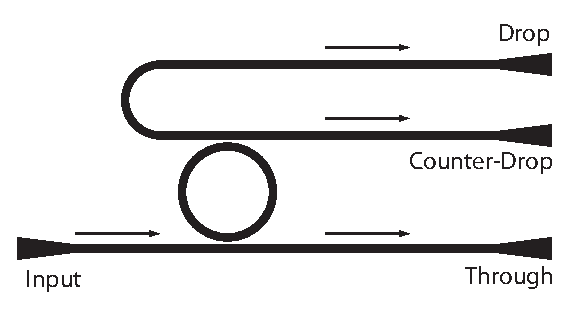
\includegraphics[width=0.45\textwidth,height=4cm]{add_drop_ring_new.eps}
    \caption{Proposed layout for future add-drop rings with drop (D), counter-drop (CD) and through (T) ports.}
    \label{fig:add_drop_ring}
\end{figure}

Figure~\ref{fig:espectro} shows the experimental result of the transmission through all three ports of one microring. It is worth noting that the shape of the resonances is very variable, even though one would expect the loss and the coupling coefficients to be approximately the same in all cases. The reason from this behavior is the backscattering parameter, which is intrinsically noisy, thus producing an apparently random response in their resonances. The backreflection is noisy because reflections are produced by lateral roughness along the ring, so they are randomly distributed along its length, and the overall reflection coefficient results from the interference of all the components, giving rise to very sharp spectral variations. In order to extract the parameters from this experimental behavior, one must take into account backreflection, otherwise the estimation of the loss and coupling coefficients would depend on which resonance we select, which is unphysical and would produce wrong results. Therefore, a procedure to extract all the parameters including backreflection is needed in order to understand the behavior of our microring resonator. Next section provides an analytical treatment and a recipe to extract all the parameters from any given resonance.


\section{Theory} 
\label{sec:theory}
A method for coupled resonators in the time domain~\cite{Haus84} was used to describe the ring, since it has already been proven to work for ring resonators were the propagating and counter-propagating are coupled through a coupling constant $u$ \cite{Zhang08}.


Following the guidelines in~\cite{Haus84,Zhang08,BLittle97-2} the following expressions for the signal in the different ports shown in Fig.~\ref{fig:add_drop_ring} are easily expressed in terms of quality factors as:
\begin{eqnarray}
	T&=& \left\lVert1-\frac{        \frac{2}{Q_{e,1}}(2j(\omega '-1)+\frac{1}{Q})   }  {   (2j(\omega '-1)+\frac{1}{Q})^2+\frac{1}{Q_u^2}  }\right\rVert^2 \label{eq:T} \\
	D &=& \left\lVert\frac{          \frac{2}{\sqrt{Q_{e,1}Q_{e,2}}}(2j(\omega '-1)+\frac{1}{Q})   }  {   (2j(\omega'-1)+\frac{1}{Q})^2+\frac{1}{Q_u^2}    }\right\rVert^2 \label{eq:D} \\
	CD&=& \left\lVert\frac{          \frac{2}{Q_u\sqrt{Q_{e,1}Q_{e,2}}}   }  {   (2j(\omega'-1)+\frac{1}{Q})^2+\frac{1}{Q_u^2}    }\right\rVert^2 \label{eq:CD}
\end{eqnarray}

%Esta figura esta puesta aqui por motivos puramente tecnicos pero aparece al comienzo de la siguiente hoja
\begin{figure*}[!t]
    \centering
    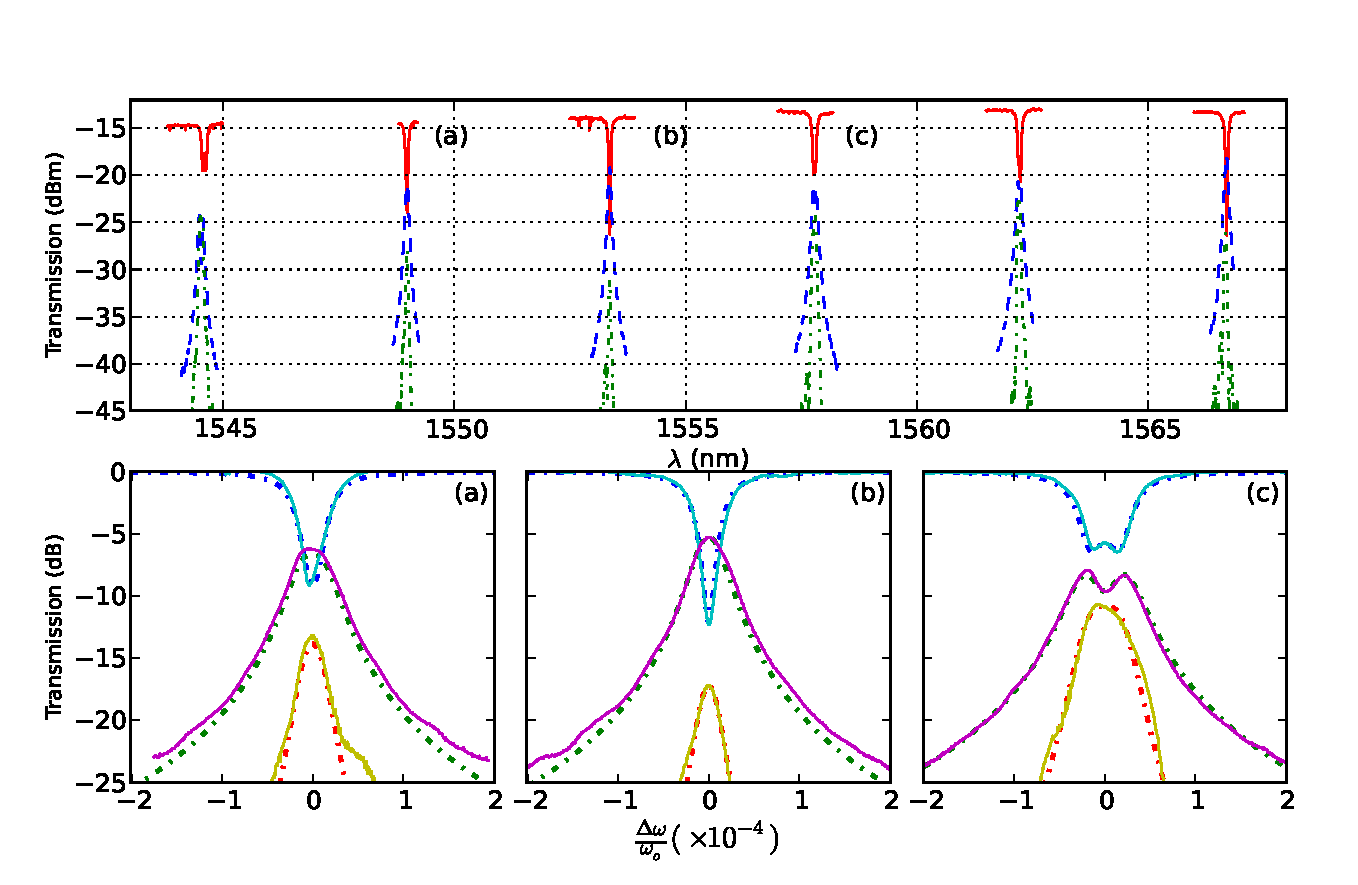
\includegraphics[width=1.0\textwidth,height=8cm]{espectro_2.eps}
    \caption{Top panel: Solid curves are measurements of the through port, while the dashed and dot-dashed lines are the drop and counter-drop ports respectively. Bottom panels: Detail of the 3 fitted resonances at 1549, 1553 and 1558 nm. All frequencies have been normalized to their resonance frequency. Solid lines are the experimental data and dashed lines are the theoretical curves using the extracted parameters shown in Table~\ref{results_table}}
    \label{fig:espectro}
\end{figure*}
%%%%%%%%%%%%%%

where $\omega'$ is the normalized angular frequency of the resonance under study, and the Q-factors are related to the $\tau$ constants of a time-domain analysis through $Q_j=\omega_o \tau_j/2$. The Q values $Q_{e,1}$, $Q_{e,2}$, $Q_{i}$ and $Q_{u}$ correspond respectively to the extrinsic coupling with the bottom and top waveguides, the intrinsic losses and the coupling constant. 

In order to extract the value of the different parameters, a measurement of the through, drop and counter-drop ports is needed. From a measurement of the three ports when $\omega'=1$ ($T_o,D_o,CD_o$) and the full width half maximum ($\delta_{FWHM}$) of the counter-drop port, the 4 parameters that characterize the ring can be deduced. These are: the energy coupling of the bottom waveguide to the ring, $k_1$, the corresponding coupling for the top guide, $k_2$, the intrinsic losses, $\alpha$, and the strength of the coupling in between the two modes. The expressions that result from particularizing equations~\ref{eq:T},\ref{eq:D} and \ref{eq:CD} for $\omega'=1$ and measuring the FWHM of the counter-drop port, are given by:
\begin{eqnarray}
    Q&=&\frac{1}{A} \label{eq:Q} \\
    Q_{e,1}&=&\frac{2A}{(A^2+u^2)(1\pm\sqrt{T_o})}  \label{eq:Qe1}\\
    Q_{e,2}&=&\frac{2A(1\pm\sqrt{T_o})}{D_o(A^2+u^2)}  \label{eq:Qe2}\\
    Q_i^{-1}&=&Q^{-1}-Q_{e1}^{-1}-Q_{e2}^{-1} \label{eq:Qi} \\
    Q_u&=&\frac{1}{u} \label{eq:Qu}
\end{eqnarray}

where:
\begin{eqnarray}
    A&=&\frac{\delta_{FWHM}}{\sqrt{\frac{CD_o}{D_o}-1 + \sqrt{\left(\frac{CD_o}{D_o}\right)^2+1}}}\\
    u&=&\sqrt{\frac{CD_o}{D_o}}A
\end{eqnarray}

where $\delta_{FWHM}$ is normalized.

The sign ambiguity in equations~\ref{eq:Qe1} and \ref{eq:Qe2} is a byproduct of the existence of two degenerate operation regimes in the ring with different parameters but the same resonance shape. This ambiguity is well known in cases without any backreflection effect, and it is usually  overcome by measuring rings with different parameters or looking at the dependence on wavelength as in \cite{McKinnon09}. In our case, the ambiguity only occurs for the peak with lowest reflection coefficient (the peak labeled as (b)), as in the other two cases it would give rise to a negative loss coefficient, which is unphysical. As the sign has to be the same in all the peaks of the same ring, this provides a way to decide the correct sign in the expressions by analysing more than one peak and looking for non-physical solutions.


Using the expressions in \cite{BLittle97-2} and $Q=\omega\tau/2$ the quality factor can be related to the usual energy coupling constants and losses by:
\begin{equation}
    K_j=\frac{\omega_oL}{Q_{e,j} v_g}  \qquad \alpha=\frac{\omega_o}{Q_i v_g} \qquad H_o=\frac{\omega_o}{2Q_uv_g}
\end{equation}


In this expression $v_g$ is the group velocity of the waveguide and can be obtained from the FSR of the ring. Finally, $Q_u$ has been related to the mean backscattered energy per unit length ($H_o$) through the group velocity $v_g$ of the waveguide, because we know from it the mean time that a photon takes to get coupled to the counter-propagating mode, $\tau_u$, and hence, reflected. It has to be remarked that although we are obtaining a distributed parameter, reflections occur at randomly localized points, being this the result of the interference that is responsible for the random nature of the variations of backscattering versus wavelength \cite{stat_backscattering}.




\section{Results}
%The measured spectra at the three ports can be seen in Fig.~\ref{fig:espectro}. As it is expected from the results in \cite{stat_backscattering}, the extinction ratios and characteristics of the different resonances show a great variability since the backscattering differs from one resonance to the next. This effect can only be observed at high Q-factors due to the increasing relative importance of $Q_u$ with respect to $Q$.

From the experimental data shown in Fig.~\ref{fig:espectro}, we have chosen three consecutive resonances which show quite different behavior in terms of extintion ratio and degree of splitting. The results obtained from the method described in section~\ref{sec:theory} for each resonance are shown in Table I, and the theoretical curves obtained from those parameters are shown in the insets of Fig.~\ref{fig:espectro}, where a good agreement is observed. It is worth noting that the coupling constants and the loss show small variations from resonance to resonance, being the backscattering coefficient the one showing strongest variations. This is expected from the nature of backscattering, and is a demonstration of the validity of our model. The asymmetry of the shape of peaks 1 and 3, which is not reproduced in the theory, could be explained by sudden variations in the reflection coefficient along the width of the resonance, which is not considered in the model.


\section{Conclusion}
We have shown an analytical model and a fitting procedure which allows to extract all the key parameters of a silicon microring resonator with two coupling points. These parameters are both coupling constants, propagation loss and the backscattering coefficient. With this method, we demonstrate that variations of the backscattering parameter are the cause of the strong variations in the shape of different resonances of the same microring. All these parameters can be extracted from simple transmission measurements.

%We think that the methods described in this paper to analyze the parameters from a ring-type resonator when high-Q factors are intended, is an improvement with respect to other methods that don't take into consideration the effects of mutual mode coupling due to backscattering in the ring. Our method also allows for a way to measure the backscattering in waveguides with a standard characterization setup.



% An example of a double column floating figure using two subfigures.
% (The subfig.sty package must be loaded for this to work.)
% The subfigure \label commands are set within each subfloat command, the
% \label for the overall figure must come after \caption.
% \hfil must be used as a separator to get equal spacing.
% The subfigure.sty package works much the same way, except \subfigure is
% used instead of \subfloat.
%
%\begin{figure*}[!t]
%\centerline{\subfloat[Case I]\includegraphics[width=2.5in]{subfigcase1}%
%\label{fig_first_case}}
%\hfil
%\subfloat[Case II]{\includegraphics[width=2.5in]{subfigcase2}%
%\label{fig_second_case}}}
%\caption{Simulation results}
%\label{fig_sim}
%\end{figure*}
%
% Note that often IEEE papers with subfigures do not employ subfigure
% captions (using the optional argument to \subfloat), but instead will
% reference/describe all of them (a), (b), etc., within the main caption.


% An example of a floating table. Note that, for IEEE style tables, the 
% \caption command should come BEFORE the table. Table text will default to
% \footnotesize as IEEE normally uses this smaller font for tables.
% The \label must come after \caption as always.
%
\begin{table}[!t]
%% increase table row spacing, adjust to taste
\renewcommand{\arraystretch}{1.3}
\label{results_table}
\centering
\begin{tabular}{|c|c|c|c|}
%\cline{2-4}
%\multicolumn{1}{l|}{}&\multicolumn{3}{c}{$\lambda$(nm)}\vline\\
%\cline{2-4}
%\multicolumn{1}{l|}{}&1549.0&1553.4&1557.8 \\
\hline
$\lambda(nm)$&1549.0&1553.4&1557.8 \\
\hline
\hline
$K_1(\%)$ & 3.35 & 3.33 & 4.18\\
\hline
$K_2(\%)$ & 1.70 & 1.76 & 1.96\\
\hline
$\alpha (dB/cm)$ & 12.4 & 11.2 & 12.7\\
\hline
$H_o (mm^{-1})$ & 0.15 & 0.08 & 0.34\\
\hline
\end{tabular}
\caption{Extracted parameters from the peaks shown in Fig.~\ref{fig:espectro}. As expected, the strongest variations are in the backreflection coefficients}
\end{table}

% use section* for acknowledgement
\section*{Acknowledgments}


The authors acknowledge financial support from the Spanish Ministry of Science and Innovation through contract SINADEC (TEC2008-06333). EPIXfab is also acknowledged for the fabrication of the devices.





% trigger a \newpage just before the given reference
% number - used to balance the columns on the last page
% adjust value as needed - may need to be readjusted if
% the document is modified later
%\IEEEtriggeratref{8}
% The "triggered" command can be changed if desired:
%\IEEEtriggercmd{\enlargethispage{-5in}}


\begin{thebibliography}{10}

\bibitem{BLittle98}
B.~E. Little, J.~Foresi, G.~Steinmeyer, et al, "Ultra-compact Si-SiO2 microring resonator optical channel dropping filters", \emph{Photonics Technology Letters, IEEE}, vol.~10, 1998, p.549-551.

\bibitem{KVos07}
K.~De Vos, I.~Bartolozzi, E.~Schacht, et al, "Silicon-on-Insulator microring resonator for sensitive and label-free biosensing", \emph{Optics Express}, vol.~22, Jan. 1997, pp.~4-6.

\bibitem{Almeida04}
V.~R.~Almeida, C.~A.~Barrios, R.~R.~Panepucci, and M.~Lipson, "All-optical control of light on a silicon chip," \emph{Nature}, vol.~431, 2004, p.~1081-1084

\bibitem{Morichetti10}
F.~Morichetti, A.~Canciamilla, M.~Martinelli, et al, "Coherent backscattering in optical microring resonators," \emph{Applied Physics Letters, }vol.~96, 2010, p. 081112.

\bibitem{BLittle97}
B.~E. Little, J.~P.~Laine, and S.~T.~Chu, "Surface-roughness-induced contradirectional coupling in ring and disk resonators," \emph{Optics letters, } vol. 22, Jan. 1997, pp. 4-6.

\bibitem{Morichetti2010}
F.~Morichetti, A.~Canciamilla, C.~Ferrari, et al, "Roughness induced backscattering in optical silicon waveguides," \emph{Physical review letters,} vol.~104, 2010, p. 33902.

\bibitem{Haus84}
H.~A.~House, "Waves and fields in optoelectronics," Ch.~7, Prentice-Hall, 1984.

\bibitem{Zhang08}
Z.~Zhang, M.~Dainese, L.~Wosinski, and M.~Qiu, "Resonance-splitting and enhanced notch depth in SOI ring resonators with mutual mode coupling," \emph{Optics Express, } vol.~16, no.~7, 2008, p.4621-4630.

\bibitem{BLittle97-2}
B.~E. Little, S.~Chu, H.~Haus, et al, "Microring resonator channel dropping filters", \emph{Journal of lightwave technology}, vol.~15, no.~16, 1997, p.998-1005.

\bibitem{McKinnon09}
W.~R.~McKinnon, D.-X.~Xu, C.~Stoney, E.~Post, et al, "Extracting coupling and loss coefficients from a ring resonator," \emph{Optics Express, } vol.~17, no~21, 2009,p.18971-18982.

\bibitem{stat_backscattering}
F.~Morichetti, A.~Canciamilla and, A.~Melloni, "Statistics of backscattering in optical waveguides", \emph{Optics Letter}, vol.~35, no.~11, 2010, p.1777-1779

\end{thebibliography}


%\begin{figure}[!h]
%    \centering
%    \includegraphics[width=1.0\textwidth]{ajuste_1549.eps}
%    \caption{Layout of the rings.}
%    \label{fig:add_drop_ring}
%\end{figure}


\end{document}
